\documentclass[english,hangout]{beamer}

\usepackage{rotating}
\usepackage{verbatim}
\usepackage{latexsym}
\usepackage{graphicx}
\usepackage{tabularx}
\usepackage{ragged2e}
\usepackage{eurosym}   % Euro symbol: \euro
\usepackage{listings}
\usepackage{multirow}
\usepackage{colortbl}
\usepackage{textcomp}  % many special symbols
\usepackage{lmodern}
\usepackage{times}
\usepackage[T1]{fontenc}
\usepackage[utf8]{inputenc}
\usepackage[english]{babel}
\usepackage{booktabs}

%\usetheme{FrankfurtUniversity}
\usetheme[fb2]{FrankfurtUniversity}

\title{Deploying Private/Hybrid Cloud \\IaaS OpenStack}
\author{Jathin Sreenivas, Vidya Gopalakrishnarao, Vineeth Bhat}
\institute{Frankfurt University of Applied Sciences}
\date{February 5, 2021}

\begin{document}
\begin{frame}
 \titlepage   
\end{frame}

\begin{frame}
   \frametitle{Agenda}
   \tableofcontents%[hideallsubsections]
\end{frame}

\section{Introduction}
\begin{frame}
    \frametitle{Introduction}
OpenStack is a free open cloud computing platform, deployed as Infrastructure-as-a-Service (IaaS), where one can provide virtual services and resources as both public and private cloud.

    
\end{frame}
\section{Architecture}
\begin{frame}
    \frametitle{Architecture}
    \begin{figure}
        \centerline{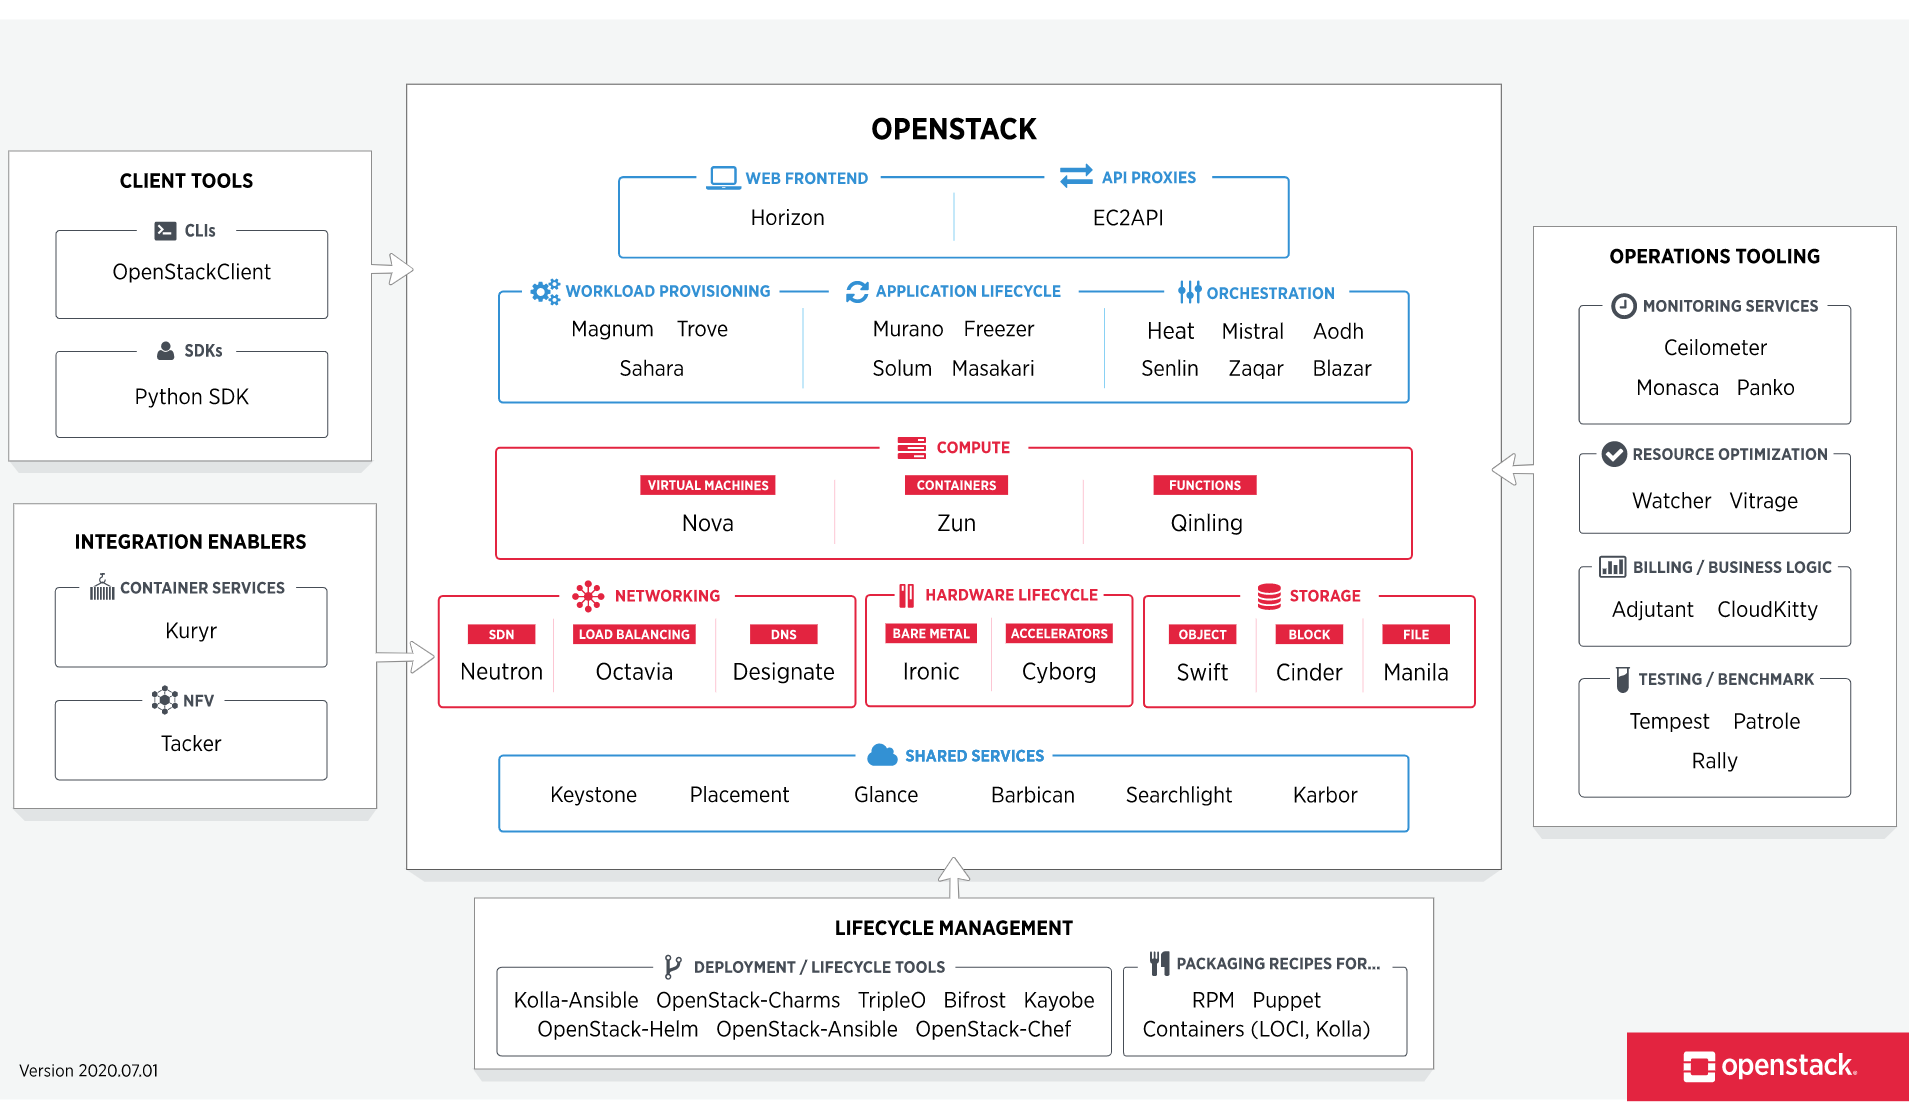
\includegraphics[height=6cm,width=11cm]{OpenStack Arch.png}}
        \caption {OpenStack Architecture \cite{b1}}
        \label{openstackArch}
    \end{figure}
\end{frame}

\subsection{Components}
\begin{frame}
    \frametitle{Components}
    \begin{figure}
        \centerline{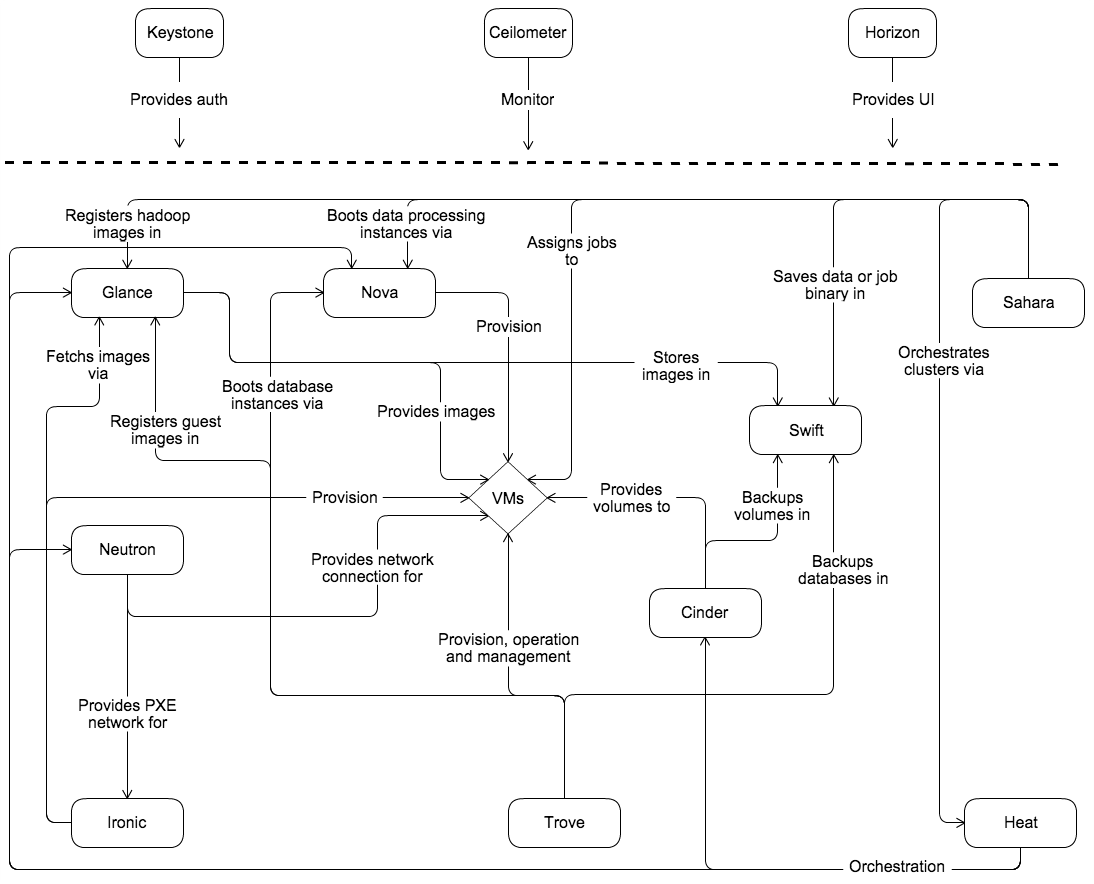
\includegraphics[height=6cm,width=10cm]{openstack_kilo_conceptual_architecture.png}}
        \caption {OpenStack Components \cite{b2}}
        \label{openstackComponents}
    \end{figure}
\end{frame}

\section{Deployment}
\subsection{Microstack}
\begin{frame}{MicroStack\cite{b3}}
\begin{itemize}
   \item MicroStack provides a single or multi-node OpenStack deployment which can run directly on your workstation.
   \item MicroStack is an OpenStack in a snap which means that all OpenStack services and supporting libraries are packaged together in a single package which can be easily installed, upgraded or removed.
   \item MicroStack includes all key OpenStack components: Keystone, Nova, Neutron, Glance, and Cinder.
   \end{itemize}
\end{frame}


\subsection{Architecture}
\begin{frame}
    \frametitle{Architecture}
    \begin{figure}
        \centerline{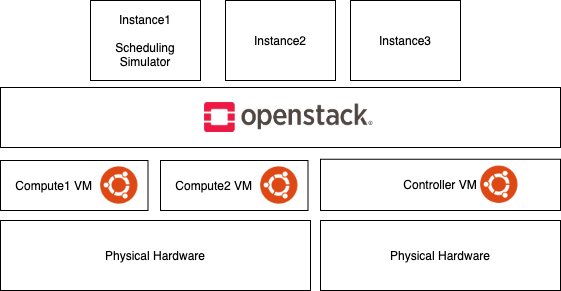
\includegraphics[height=4.5cm,width=8cm]{Architecture.png}}
        \caption {Architecture}
        \label{architecture}
    \end{figure}
\end{frame}

\subsection{Network Topology}
\begin{frame}
    \frametitle{Network Topology}
    \begin{figure}
        \centerline{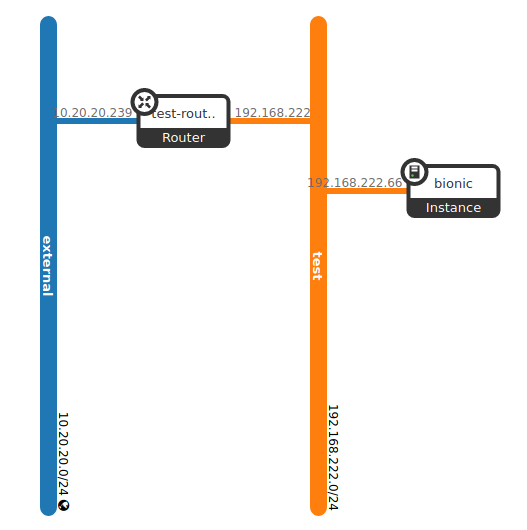
\includegraphics[height=6cm,width=7cm]{Topology.png}}
        \caption {Network Topology}
        \label{openstackComponents}
    \end{figure}
\end{frame}

\section{Demo}
\begin{frame}[fragile]
 \frametitle{Demo}
    \begin{center}
        \vspace{-1.2em}
            Demo \cite{b4}
        \end{center}
\end{frame}



\section{References}
\begin{frame}{References}
\begin{thebibliography}{00}
   \tiny \bibitem{b1} https://www.openstack.org/software/ Accessed: 4.02.2021
   \tiny \bibitem{b2} https://docs.openstack.org/install-guide/get-started-conceptual-architecture.html Accessed: 4.02.2021
   \tiny \bibitem{b3} https://ubuntu.com/tutorials/microstack-get-started#1-overview/ Accessed: 4.02.2021
   \tiny \bibitem{b4} Video is available at https://drive.google.com/drive/folders/1rVeC4K7UPgLwVmbEG3e8htqGc48ldve7?usp=sharing Accessed: 4.02.2021
\end{thebibliography}
    
\end{frame}


\end{document}